\documentclass[a4paper, 11pt]{article}
\usepackage[left=2cm,text={17cm, 24cm},top=3cm,left= 2cm]{geometry}
\usepackage[IL2]{fontenc}
\usepackage[czech]{babel}
\usepackage[utf8]{inputenc}
\usepackage{graphicx}
\usepackage[export]{adjustbox}
\usepackage{subcaption}
\usepackage{float}
\usepackage{url}
\providecommand{\uv}[1]{\quotedblbase #1\textquotedblleft}
\DeclareUrlCommand\url{\def\UrlLeft{<}\def\UrlRight{>} \urlstyle{tt}}

\begin{document}
\thispagestyle{empty}
\begin{center}
\Huge
\textsc{Vysoké učení technické v Brně}\\
\huge
\textsc{Fakulta informačních technologií}\\
\LARGE
\vspace{\stretch{0.382}}
Modelování a simulace - 6. Počítačové služby\\ \Huge Porovnávání SQL a JAVA přístupů do databáze
\vspace{\stretch{0.618}}
\end{center}

{
\LARGE \hfill
Vojtěch Meluzín - xmeluz04\\
\today \hfill
Matěj Mlejnek - xmlejn04}

\newpage
\thispagestyle{empty}

\tableofcontents

\newpage
\setcounter{page}{1}
\section{Úvod}
V této práci je řešen projekt do předmětu \textbf{IMS - Modelování a simulace} \cite{ims_web} vyučovaném na Fakulta informačních technologií Vysokého učení technického v Brně \cite{fit_web}. Konkrétně se jedná o zadání \textbf{6. Počítačové služby} \cite{zadani_web}.

Tato práce se věnuje problematice doby vyhledávání v databázi. Zaměříme se na porovnávání přístupu do databáze výhradně přes SQL dotazy a přístupu do databáze spojeného s cacheováním (jednotlivých řádků vyhledávané tabulky) na počítači klienta.

V našich experimentech se zaměřujeme zjištění za jakých podmínek je efektivnější pro vyhledávání použit spíše databázový server a nebo ve veškerých datech vyhledávát až na straně klienta. Vzhledem k tomu, že na tyto časy hraje roli několik faktorů výběr nemusí být na první pohled hned jasný. V kapitole Experimenty (viz.   Experimenty) jsou sepsány jednotlivé krajní i více obecné (realističtější) případy při práci s databází. 


\section{Zdroje faktů}
Jako model jsme si vybrali databázi Postgresql ve verzi 9.5.10 \cite{postgresql_web}. Pro přístup do této databáze jsme zvolili naprogramování aplikace v jazyce JAVA \cite{java_web} ve verzi JDK-1.8.0\_151 \cite{java_jdk_version}, ve které jsme si naprogramovali komunikaci se serverem. Programy pro sběr dat z této komunikace běželi na virtualním stroji Ubuntu 16.04.3 LTS \cite{ubuntu_web} a samotné posílání jednotlivých dotazů bylo zautomatizované pomocí scriptu psaném v GNU Bash version 4.3.48(1)-release (x86\_64-pc-linux-gnu) \cite{bash_web}.

\subsection{Průběh sběru dat}
Pro přístup k datům z databáze a měření doby přístupu k datům, jsme se rozhodli, že bude vhodné, aby se vyhledávací dotazy vytvářeli na virtuální počítači odděleného od virtuálního počítače s databázovým serverem. Vytvořili jsme tedy 2 virtuální počítače s těmito parametry: 

\begin{center}
\begin{tabular}{ |l|l| }
  \hline
  \multicolumn{2}{|c|}{VM1SERVER} \\
  \hline
  CPU & 2 jádra - 4,2 GHz \\
  RAM & 2048 MB \\
  SSD & 25 GB\\
  OS & Ubuntu - 16.04.3\\
  \hline
\end{tabular}

\hspace{20 in}

\begin{tabular}{ |l|l| }
  \hline
  \multicolumn{2}{|c|}{VM2CLIENT} \\
  \hline
  CPU & 2 jádra - 4,2 GHz \\
  RAM & 8192 MB \\
  SSD & 25 GB\\
  OS & Ubuntu - 16.04.3\\
  \hline
\end{tabular}
\end{center}
Parametry byli vybrány, tak aby splňovali minimální systémové požadavky a zároveň bylo co nejvíce místa pro nacachování prohledávaných tabulek.


Tyto parametry jsme zvolili, tak aby splňovali požadavky operačního systému Ubuntu \cite{ubuntusysreq}, databázového serveru Postgresql \cite{postgresqlsysreq} a zároveň aby se na straně klienta spustila JAVA s námi vybranými velikostmi RAM pro měření.  Virtualní diskové prostory byli fyzicky uloženy na SSD disku, který během testování nepřesáhl 20\% zatížení. 
\paragraph{OS parametry} \label{sec:os}
Operační systém ubuntu \cite{ubuntu_web} jsme si vybrali z důvodu jednoduché instalace jednotlivých aplikací potřebných pro tento sběr dat, nízké náročnosti na hardwarové požadavky a jednoduchou obsluhu.
Jako databázový systém nám posloužil PostgreSQL \cite{postgresql_web}. Tento systém jsme zvolili z důvodu jednoduché instalace, nízkých nároků na hardware a The PostgreSQL Licence(mirně modifikované Open Source licence) \cite{postgresqllicence}. Při výběru s jakou databází budeme pracovat jsme si nezvolili Oracle \cite{oracle} z důvodu, že již není volně k dispozici pro komerční použití a naše výsledky by nebyli dostatečně využitelné. 



Na prvním virtuálním počítači běžel server (dále jen VM1SERVER) s databází PostgreSQL a měl za úkol zpracovávat přijaté SQL dotazy a odpovídat na ně.
Druhý virtuální počítač znázorňující klienta (dále jen VM2CLIENT) se postupně připojoval na databázový server a posílal dotazy. 

Na VM2CLIENT tedy běžel BASH \cite{bash_web} script \textit{functions.sh}, který automaticky spouštěl námi naprogramované Javové dotazy z \textit{/dist/testApp.jar}.

V rámci automatických testů se také před každým měřením musel zaslat požadavek pro vymazání cache paměti v databázi na straně serveru, toto je vyřešeno připojením přes OpenSSH rozhrani (OpenSSH\_7.2p2 Ubuntu-4ubuntu2.4, OpenSSL 1.0.2g  1 Mar 2016) \cite{openssh} \textit{sshclear.sh} připojením se na VM1SERVER a odtud zavoláním scriptu \textit{clearcache.sh}.

\subsubsection{Přesnost vyhledávání}

Jako hodnotu pro vyhledávání jsme si zvolili index(od 1 do velikosti tabulky po 1). Rozhodli jsme se filtraci provádět podle začátku řetězce jeho hodnoty. Tato filtrace byla zvolena z toho důvodu, že se nejvíce podobá přístupu do databáze k vyhledání určité položky, aneb jak s databází pracuje normální uživatel. Při práci s databázi byla tato filtrace prováděna příkazem LIKE 'prefix\%' \cite{sqllike} a v JAVA startsWith(String prefix) \cite{javalike} (dále se na obě funkce budeme zároveň odkazovat jako na pseudofunkci LIKEE(prefix)).
\\
Příklady LIKEE() nad řetězci:
$$LIKEE("AH") > ("AHOJ") => True$$
$$LIKEE("1") > ("10") => True$$
$$LIKEE("0") > ("10") => False$$
$$LIKEE("1") > ("1") => True$$
\\
Jelikož v našem projektu pracujeme s indexovanými tabulkami, tak můžeme vyhledávat počet výskytů indexů se stejným začátkem:
$$LIKEE("1") > TABLE(100) => 12$$
$$LIKEE("1") > TABLE(1000) => 111$$
$$LIKEE("10") > TABLE(1000) => 2$$
$$LIKEE("10") > TABLE(500)=> 11$$
$$LIKEE("100") > TABLE(100)=> 1$$
$$LIKEE("100") > TABLE(30000) => 111$$
$$LIKEE("1000") > TABLE(500) => 0$$

\subsubsection{RAM pamět}
Pro výběr s jakými hodnoty RAM paměti budeme pracovat jsme byli limitování fyzickým hardwarem, proto jsme na VM1SERVER usoudili, že nebude potřeba větší než minimální Systémem a Databází požadovaná viz: \textbf{OS parametry} \ref{sec:os}. Pro VM2CLIENT jsme měli 8GB paměti. Nyní stačilo vyhledat pro jaké RAM paměti nám JAVA běžící na VM2CLIENT dovolí s maximální velikostí tabulek. Zjistili jsme, že pro JAVA při paměti 512MB dokáže nad našími tabulkami(ve formátu viz: \ref{sec:table}) pracovat s maximálně 150 000 tabulkami. Na konec jsme zvolili RAM 1024, 2048 a 4096. Tyto RAM paměti bez problému pojmou i naši největší zvolenou tabulku (250 000).

\subsubsection{Vygenerování databáze} \label{sec:table}

Pro generaci potřebných dat jsme si vybrali csv generátor \cite{csvgenerator} jednotlivé řádky jsme se rozhodli selectovat pomocí indexu("seq"), bylo ovšem zapotřebí, aby se tabulka podobala tabulkám se kterými se pracuje v reálném životě, proto jsme si zvolili, že každý řádek bude obsahovat hodnoty pro tyto sloupce:
$$"seq, first, last, age, street, city, state, zip, $$
$$dollar, pick, date, email, digid, latitude, longitude, $$
$$pick2, string, domain, float, ccnumber, bool, yn"$$
Například:
$$1,Jesse,Watts,51,Husfo Terrace,Livemil,HI,75091,\$2932.33,$$
$$YELLOW,7/13/1993,sajuvubug@uj.net,$$
$$147889110758,12.63144,-166.12131,UP,W4P9nY0yubdKsQu)sxI,$$
$$boto.co.uk,-275370638258.9952,6304284025402256,true,N$$


Velikost jednotlivých řádků tabulek by neměla ovlivnit poměr časů vyhledávání, ale slouží k tomu, aby jsme vygenerovali vstupní data k simulaci ve kterých uvidíme větší hodnoty s menší pravděpodobností vzniklých nepřesností.

Tyto data jsme umístili na VM1SERVER, tak že jsme na něm spustili databázi a připojili jsme se na ní pomocí PG ADMIN 3 \cite{pgadmin} a nahráli zde tabulky ze kterých jsme plánovali získávat data.
\paragraph{Tabulky}
Původně jsme plánovali pracovat s tabulkami velkými až 10 000 000, to jsme ovšem velice rychle zavrhli z důvodu velké časové náročnosti výpočtů. Nakonec jsme pracovali s tabulkami do velikosti 250 000.

\subsubsection{Automatizace pomocí BASH}
Z bash scriptu byl volán JAVA program [link] postupně po jednom tak aby byla provedena kombinace všech vstupních parametrů z předchozí sekce(RAM, TABLES,LIKEE). Naměřené hodnoty jsme ukládali do formátu csv. Při 
\subsubsection{Naměření hodnot JAVA}
Pro získávání dat jsme vytvořili program v jazyce JAVA (viz.\textit{/dist/testApp.jar}). V tomto programu spuštěném na VM2CLIENT se připojujeme na databázový server Postgresql běžícím na VM1SERVER. Naměřili jsme si tyto hodnoty:

\begin{itemize}
\item Doba selectu z db bez cache
\item Doba selectu z db s cache
\item Doba selectu z db bez cache a s filtrací
\item Doba selectu z db s cache a s filtraci
\item Doba vytvoření objektů v JAVA
\item Doba filtrace v JAVA

\end{itemize}
 
\subsubsection{Zpracování naměřených hodnot}
Výstupní \textit{csv} soubory jsme si prevedli do tabulkového formatu \textit{xlsx} pomocí aplikace Microsoft Excel \cite{excel}, kde jsme nad jednotlivými časy vytvářeli grafy. Na obrázku číslo \ref{sec:obr1} můžete vidět dobu vytváření objektů všech prvků z tabulky na základě její velikosti. Z grafu je jasně vidět, jak se jednotlivé časy mění při změně velikosti tabulky. 


\begin{figure}[H]
\centering
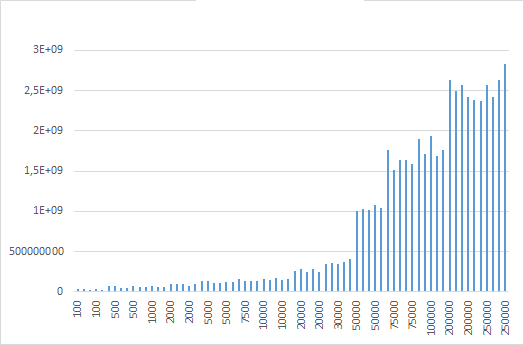
\includegraphics[width=150mm, frame]{images/LIKEE-1-CREATE-ALL.png}
\caption{LIKEE-1-CREATE-ALL - 5x měřená hodnota pro každou velikost tabulky - Vertikální osa značí čas v nanosekundách a horozontální značí velikost tabulky.}
\label{sec:obr1}
\end{figure}

\begin{figure}[H]
\centering
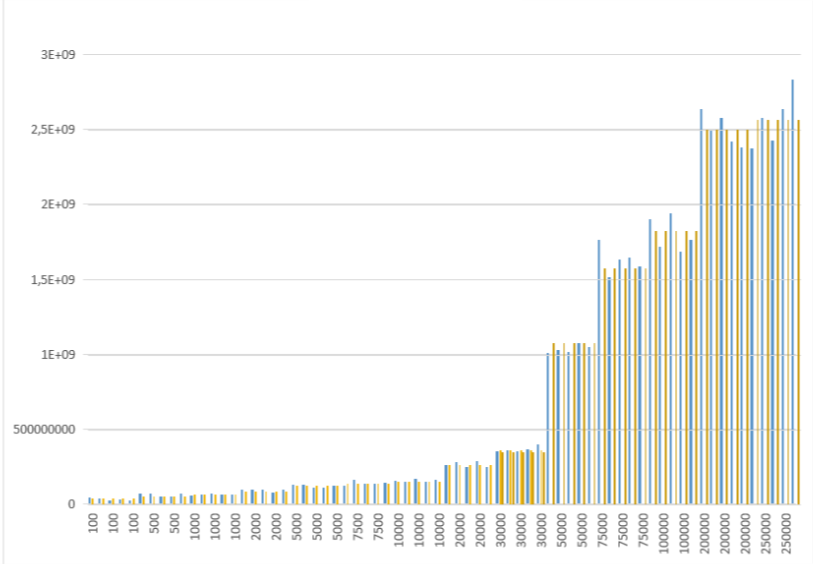
\includegraphics[width=150mm, frame]{images/LIKEE-1-CREATE-ALL-FUNCTIONS.png}
\caption{LIKEE-1-CREATE-ALL-FUNCTIONS - 5x měřená hodnota pro každou velikost tabulky - Vertikální osa značí čas v nanosekundách a horozontální značí velikost tabulky.}
\label{sec:obr2}
\end{figure}

\paragraph{Normální rozložení} Potřebovali jsme na základě těchto hodnot vytvořit funkce podle kterých, by jsme mohli určit přibližnou hodnotu různě velkých tabulek, pro které nemáme hodnoty naměřené. Na základě měření jsme rozhodli, že veškeré měřené hodnoty mají normálního rozložení (například tabulka o velikosti 100, nad kterou byl volán Select všech rádků (viz. obrázek \textbf{č. \ref{sec:obr3})}.
U každého jednotlivého grafu znázorňující naměřené hodnoty (viz. obrázek\ref{sec:obr1}) bylo zapotřebí zvážit zda není vhodné ho rozdělit na více intervalů, kde by  vytvořená funkce počítala přesněji. Z hodnot ze zvoleného intervalu jsme přes online nástroj pro vytváření polynomu viz. \cite{polregres} vždy získali dány polynom většinou čtvrtého řádu, do kterého jsme potom dosadili původní velikosti tabulek. Původní graf hodnot a hodnoty z nových funkcí jsme si dali dohromady do grafu na porovnání. Na obrázku číslo \ref{sec:obr2} můžeme vidět jak žlutá barva znázorňuje body spočítané z nově vytvořených funkcí. 


\begin{figure}[H]
\centering
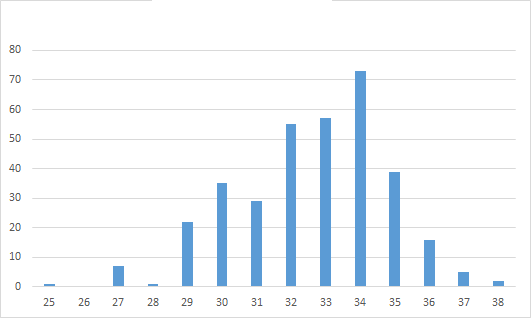
\includegraphics[width=150mm, frame]{images/100-TABLE-SELECT-ALL-342.png}
\caption{100-TABLE-SELECT-ALL - rozložení při 342 měřeních - vertikální osa značí počet výskytů a horozontální značí $10^{-2}$ sekund zaokrouhleno na celá čísla}
\label{sec:obr3}
\end{figure}


\paragraph{rozptyl} Pro jednotlivé intervaly jsme si u každého bodu co jsme měli naměřenou hodnotu spočítali hodnotu funkce, a tím zjistili chybu v jednotlivých bodech. Tyto chyby stačilo zprůměrovat a získali jsme hodnotu rozptylu. 
\paragraph{DX - odchylka} Z vypočítaného rozptylu odečítáme jednotlivé časy 
\paragraph{EX - Střední hodnota} Střední hodnotu jsme zjistili z četnosti výskytů hodnot na intervalu \ref{sec:obr3}) pro danou vytvořenou funkce.
 ????????????????????????????? 
https://matematika.cz/smerodatna-odchylka
??????????????
nope my jsme vzali ty body na těch intervalech a aproximovali jsme je. Pak z té aproximace vypadla funkce. Tu funkci jsme pak použili na vypočítání EX a od toho EX jsme pak udělali průměrnou odchylku, kterou jsme použili jako rozptyl.
Chtělo by to tam pak i přidat ty vzorečky jak máme
na normální rozdělení


\begin{figure}[H]
\centering
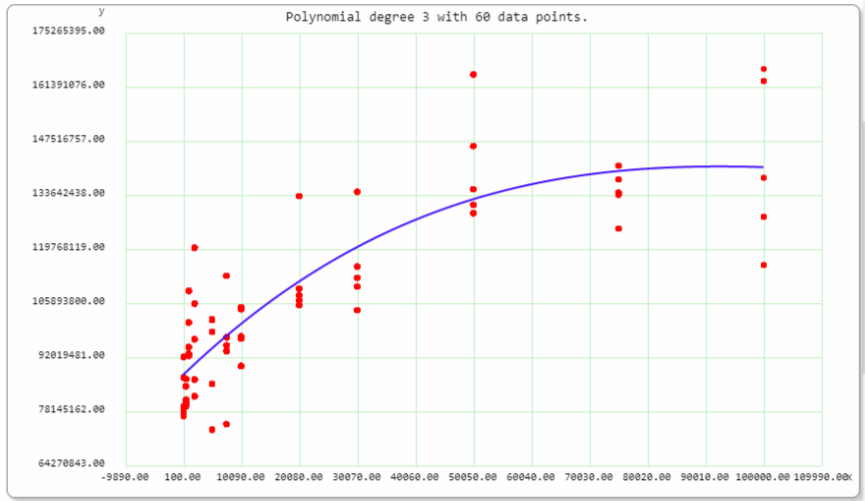
\includegraphics[width=150mm, frame]{images/VYPOCET-KRIVEK.png}
\caption{pres reference https://arachnoid.com/polysolve/}
\label{sec:obr9}
\end{figure}

\subsection{Ověření funkčnosti modelu}
Validita modelu byla ověřována porovnáváním dat, které jsme vygenerovali s daty naměřenými.

analyzujeme a modelujeme v simlibu\cite{simlib_web, simlib_zdroj}

\begin{figure}[H]
\centering
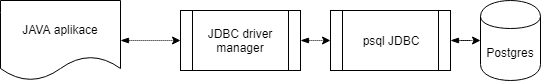
\includegraphics[width=150mm]{images/JAVA-DB-komunikace.png}
\caption{Komunikace JAVA-DB}
\label{sec:obr8}
\end{figure}



\subsection{Petriho sít}

\begin{figure}[H]
\centering
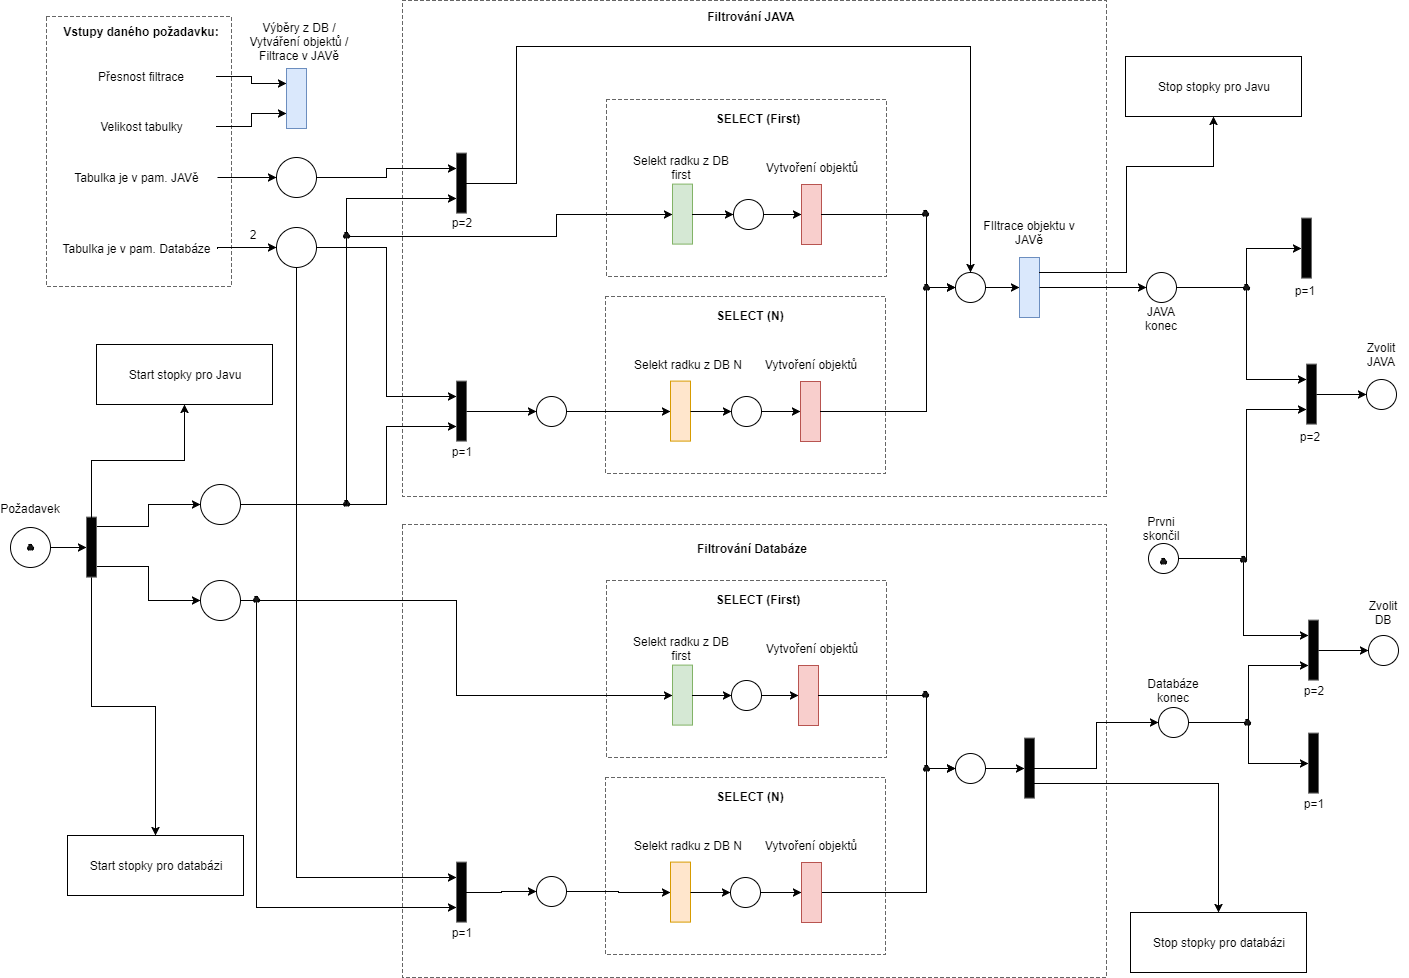
\includegraphics[width=220mm,  angle =90]{images/IMS-projekt.png}
\caption{Petriho sít}
\label{sec:obr7}
\end{figure}

\section{Experimenty}


\begin{figure}[H]
\centering
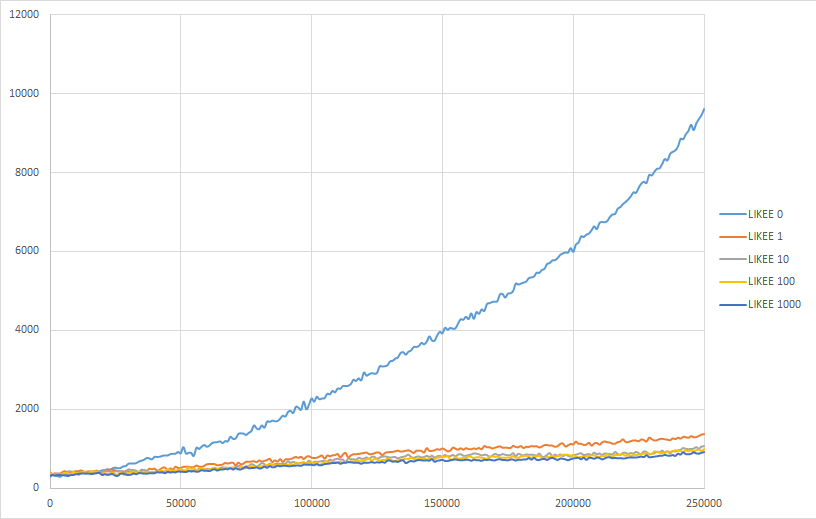
\includegraphics[width=150mm, frame]{images/FIRST-DB.png}
\caption{FIRST - DB - LIKEE 0-1-10-100-1000 - Vertikální osa čas $10^{-3}$ sekund a horozontální značí velikost tabulek.}
\label{sec:obr5}
\end{figure}

\begin{figure}[H]
\centering
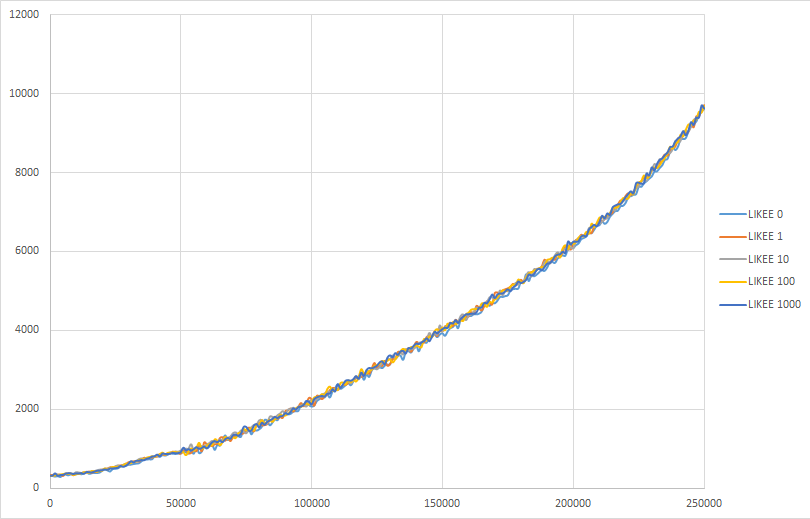
\includegraphics[width=150mm, frame]{images/FIRST-JAVA.png}
\caption{FIRST - JAVA - LIKEE 0-1-10-100-1000 - Vertikální osa čas $10^{-3}$ sekund a horozontální značí velikost tabulek.}
\label{sec:obr6}
\end{figure}

\begin{figure}[H]
\centering
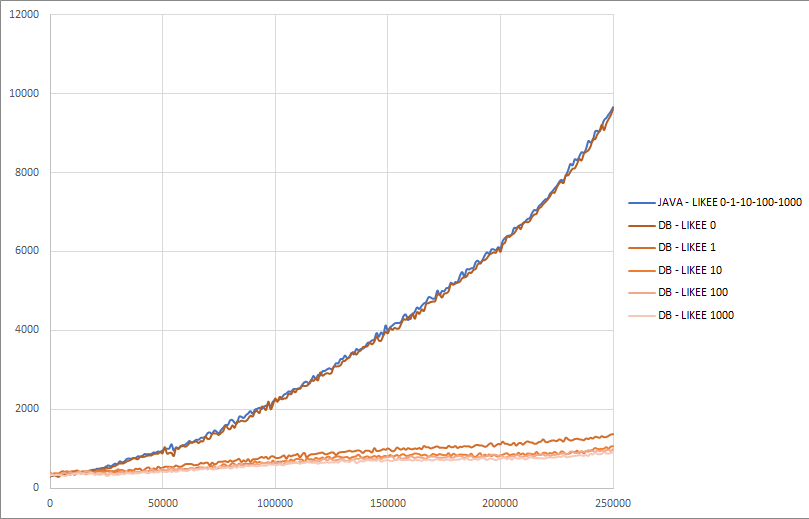
\includegraphics[width=150mm, frame]{images/FIRST-DB-JAVA-INTERSECTION.png}
\caption{FIRST - DB AND JAVA - LIKEE 0-1-10-100-1000 TABLE 0-40000 - Vertikální osa čas $10^{-3}$ sekund a horozontální značí velikost tabulek.}
\label{sec:obr4}
\end{figure}



\section{Závěr}

//RAM STUFFFF

Potom nějaká věta o tom, že v naměřených datech, jsme zjistili, že nakonec měla RAM jen (určitý vliv) a to jen u vybírání celých nebo jen likee 1 filtraci

Pozn. Pokud používáme přesné filtrování pomocí databáze, tak bychom mohli i pro větší tabulky zvolit menší RAM. 


\pagebreak
\newpage
\bibliographystyle{czechiso}
\def\refname{Literatura}
\bibliography{proj4}

\end{document}